\begin{figure}[h!]
\textbf{Tema d'Esame di Gennaio 2015}\\ \\
Si determini la differenza di potenziali ai capi della resistenza $R4$ del circuito mostrato in figura. La differenza di potenziale fornita dalla batteria è di $12V$ e i valori delle resistenze sono rispettivamente $R2=15\Omega, R3=40\Omega, R4=25\Omega, R5=R6=32\Omega, R1=R7=18\Omega$
\begin{center}
		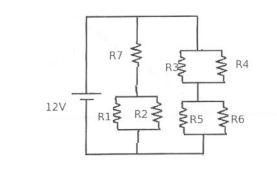
\includegraphics[scale=1.2]{ES5/GEN052015.jpg}
	\end{center}

	\noindent\fbox{
		\parbox{\textwidth}{
			\null\hfill \textbf{Soluzione:} $V_4 = 5.85 V$\\
			\textbf{Procedimento: } \\
			Semplificazione delle Resistenze:\\
			$R_{34}=\frac{R_3\cdot R_4}{R_3+R_4}=\frac{40\Omega \cdot 25\Omega}{40\Omega+25\Omega}=15.38\Omega$\\
			$R_{56}=\frac{R_5\cdot R_6}{R_5+R_6}=\frac{32\Omega \cdot 32\Omega}{32\Omega+32\Omega}=16\Omega$\\
			$R_{12}=\frac{R_1\cdot R_2}{R_1+R_2}=\frac{18\Omega \cdot 15\Omega}{18\Omega+15\Omega}=8.18\Omega$\\
			$R_{127}=R_{12}+R_7=8.18\Omega + 18\Omega=26.18\Omega$\\
			$R_{3456}=R_{34}+R_{56}=15.38\Omega+16\Omega=31.38\Omega$\\
			$R_{tot}=\frac{R_{127}\cdot R_{3456}}{R_{127}+R_{3456}}=\frac{26.18\Omega \cdot 31.38\Omega}{26.18\Omega + 31.38\Omega}=14.23\Omega$\\ \\
			Ricordando che la tensione in parallelo non cambia, così come non cambia la corrente in serie:\\
			$V_{tot}=V_{127}=V_{3456}=12V$\\
			$I_{3456}=\frac{V_{3456}}{R_{3456}}=0.38A \qquad I_{3456}=I_{34}=I_{56}$\\
			$V_{34}=V_3=V_4=R_{34}\cdot I_{34}=15.38\Omega \cdot 0.38A=5.85\Omega \qquad V_{34}=V_3=V_4$
		}
	}	
	
\end{figure}

\begin{figure}[h!]
\textbf{Tema d'Esame di Febbraio 2015}\\ \\
 Nel circuito in figura, la corrente attraverso $R6$ è $i_6=1.40A$ e le resistenze sono
$R1=R2=R3=2.0\Omega, R4= 16.0\Omega, R5= 8.0 \Omega , R6= 4.0 \Omega$. Qual'è la forza elettromotrice della batteria (ideale)?
\begin{center}
		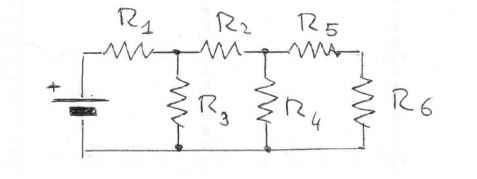
\includegraphics[scale=0.8]{ES5/FEB052015.jpg}
	\end{center}

	\noindent\fbox{
		\parbox{\textwidth}{
			\null\hfill \textbf{Soluzione:} $V = 48.3 V$\\
			\textbf{Procedimento: } \\
			Ricordando che la tensione in parallelo non cambia, così come non cambia la corrente in serie proseguiamo semplificando le resistenze e aggiornando man mano corrente e tensione:\\
			$R_{56}=R_5 + R_6=8\Omega + 4\Omega=12\Omega$\\
			$V_{56}=R_{56}\cdot I_6=16.8V$\\\\
			$R_{456}=\frac{R_{56}\cdot R_4}{R_{56}+R_4}=\frac{12\Omega\cdot 16\Omega}{12\Omega + 16\Omega}=6.85\Omega$\\
			$I_{456}=\frac{V_{56}}{R_{456}}=\frac{16.8V}{6.85\Omega}=2.45A$\\ \\
			$R_{2456}=R_2+R_{456}=2\Omega+6.85\Omega=8.85\Omega$\\
			$V_{2456}=R_{2456}\cdot I_{456}=8.85\cdot 2.45A=21.68V$\\ \\
			$R_{23456}=\frac{R_3\cdot R_{2456}}{R_3+ R_{2456}}=\frac{2\Omega \cdot 8.85\Omega}{2\Omega+ 8.85\Omega}=1.63\Omega$\\ \\
			$I_{23456}=I_{tot}=\frac{V_{23456}}{R_{23456}}=\frac{21.68V}{1.63\Omega}=13.3A$\\
			$R_{tot}=R_1+R_{23456}=2\Omega+1.63\Omega=3.63\Omega$\\
			$V=R_{tot}\cdot I_{tot}=3.63\Omega \cdot13.3A=48.28V$
		}
	}	
\end{figure}

\begin{figure}[h!]
\textbf{Tema d'Esame di Giugno 2015}\\ \\
Si determini la differenza di potenziali ai capi della resistenza R4 del circuito mostrato in figura. La differenza di potenziale fornita dalla batteria è di $12V$ e i valori delle resistenze sono rispettivamente $R2=15\Omega, R3=40\Omega, R4=25\Omega, R5=R6=32\Omega, R1=R7=18\Omega$.
	\begin{center}
		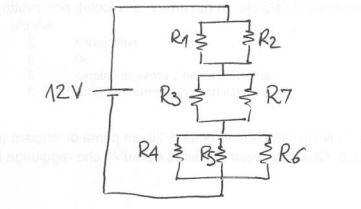
\includegraphics[scale=1]{ES5/GIU052015.jpg}
	\end{center}

	\noindent\fbox{
		\parbox{\textwidth}{
			\null\hfill \textbf{Soluzione:} $V_4 = 3.85 V$\\
			\textbf{Procedimento: } \\
			Semplificazione delle Resistenze:\\
			$R_{12}=\frac{R_1\cdot R_2}{R_1+R_2}=\frac{18\Omega \cdot 15\Omega}{18\Omega+15\Omega}=8.18\Omega$\\
			$R_{37}=\frac{R_3\cdot R_7}{R_3+R_7}=\frac{40\Omega \cdot 18\Omega}{40\Omega+18\Omega}=12.41\Omega$\\
			$R_{456}=\frac{1}{\frac{1}{R_4}+\frac{1}{R_5}+\frac{1}{R_6}}=\frac{1}{\frac{1}{25\Omega}+\frac{1}{32\Omega}+\frac{1}{32\Omega}}=9.76\Omega$\\
			$R_{tot}=R_{12}+R_{34}+R_{456}=8.18\Omega+12.41\Omega+9.76\Omega=30.35\Omega$\\
			Ricordando che la tensione in parallelo non cambia, così come non cambia la corrente in serie:\\
			$I_{tot}=I_{12}=I_{34}=I_{456}=\frac{V}{R_{tot}}=\frac{12V}{30.35\Omega}=0.395A$\\
			$V_4=V_5=V_6=R_{456}\cdot I_{tot}=9.76\Omega\cdot 0.395A=3.85V$
		}
	}	
	
\end{figure}

\begin{figure}[h!]
\textbf{Tema d'Esame di Luglio 2015}\\ \\
Si determini la differenza di potenziale ai capi della resistenza $R_4$ nel seguente circuito. La differenza di potenziale fornita dalla batteria è di $12V$ e i valori delle resistenze sono rispettivamente $R2=15\Omega, R3=40\Omega, R4=25\Omega, R5=R6=32\Omega, R1=R7=18\Omega$
	\begin{center}
		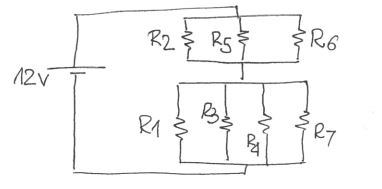
\includegraphics[scale=1]{ES5/LUG052015.jpg}
	\end{center}

	\noindent\fbox{
		\parbox{\textwidth}{
			\null\hfill \textbf{Soluzione:} $V_4 = 5.05 V$\\
			\textbf{Procedimento: } \\
			Semplificazione delle Resistenze:\\
			$R_{256}=\frac{1}{\frac{1}{R_2}+\frac{1}{R_5}+\frac{1}{R_6}}=\frac{1}{\frac{1}{15\Omega}+\frac{1}{32\Omega}+\frac{1}{32\Omega}}=7.74\Omega$\\\\
			$R_{1347}=\frac{1}{\frac{1}{R_1}+\frac{1}{R_3}+\frac{1}{R_4}+\frac{1}{R_7}}=\frac{1}{\frac{1}{18\Omega}+\frac{1}{40\Omega}+\frac{1}{25\Omega}+\frac{1}{18\Omega}}=5.68\Omega$\\ \\ 
			$R_{tot}=7.74\Omega+5.68\Omega=13.42\Omega$\\ \\
			Ricordando che la tensione in parallelo non cambia, così come non cambia la corrente in serie:\\
			$I_{tot}=I_{256}=I_{1347}=\frac{V}{R_{tot}}=\frac{12V}{13.42\Omega}=0.89A$\\
			$V_4=V_1=V_3=V_7=R_{1237}\cdot I_{tot}=5.68\Omega\cdot 0.89A=5.05V$
		}
	}	
	
\end{figure}